\subsection{Detection Subsystem}
\noindent Recall the requirements of the detection subsystem. It should be able to detect objects at least 3 meters away and within a 15 degree aspect angle. It also should detect walker instability up to 10 degrees in pitch angle. It should detect hazards with an accuracy of at least 80\%. Finally, feedback latency should not exceed 100 milliseconds to keep the user safe.\\

\noindent Let us also define the input and output of the obstacle detection subsystem. The input is energy return from the environment, supplied to 5 different points on the walker frame, as well as accelerometer and magnetometer data outputs describing the attitude of the walker itself. The output is somewhat joint with the obstacle identification system, as it helps to generate velocity motor commands for both speed and turn angle. Detection and identification are the FORWARD system inputs, and avoidance is the output.\\

\subsubsection{I2C Bus for Sensors}
\noindent The utilization of 4 ultrasonic sensors and 1 LiDAR to supply a feed of information to FORWARD's central processor can be integrated and realized through a wiring bus with the I2C digital communication protocol. This I2C scheme will use a synchronous clock signal provided to the sensors by the MCU. It will operate always in half-duplex, meaning data will be transmitted in only one direction at a time - from the MCU to the sensors and from the sensors back to the MCU in successive time steps. Additionally, the sensors will be accessed by their unique addresses and send packets of information as a sequence, taking turns.\\

\subsubsection{Sensor Orientation}
\noindent The range sensors are mounted on the frame perpendicularly to obstacles. In other words, the direction of the energy transmitted is perpendicular to the ground. However, the question of maximizing capability of detecting obstacles at the wheel level, and to prevent ignorance of more dangerous and deceptive hazards such as ledges or step-downs is raised.\\

\subsubsection{Incline and Decline Stability}
\noindent The simple function fulfilled by the inclusion and integration of the IMU is stability. By monitoring the pitch angle of the walker, we know whether the user is at risk of falling over.\\

\begin{figure}[H]
	\centering
	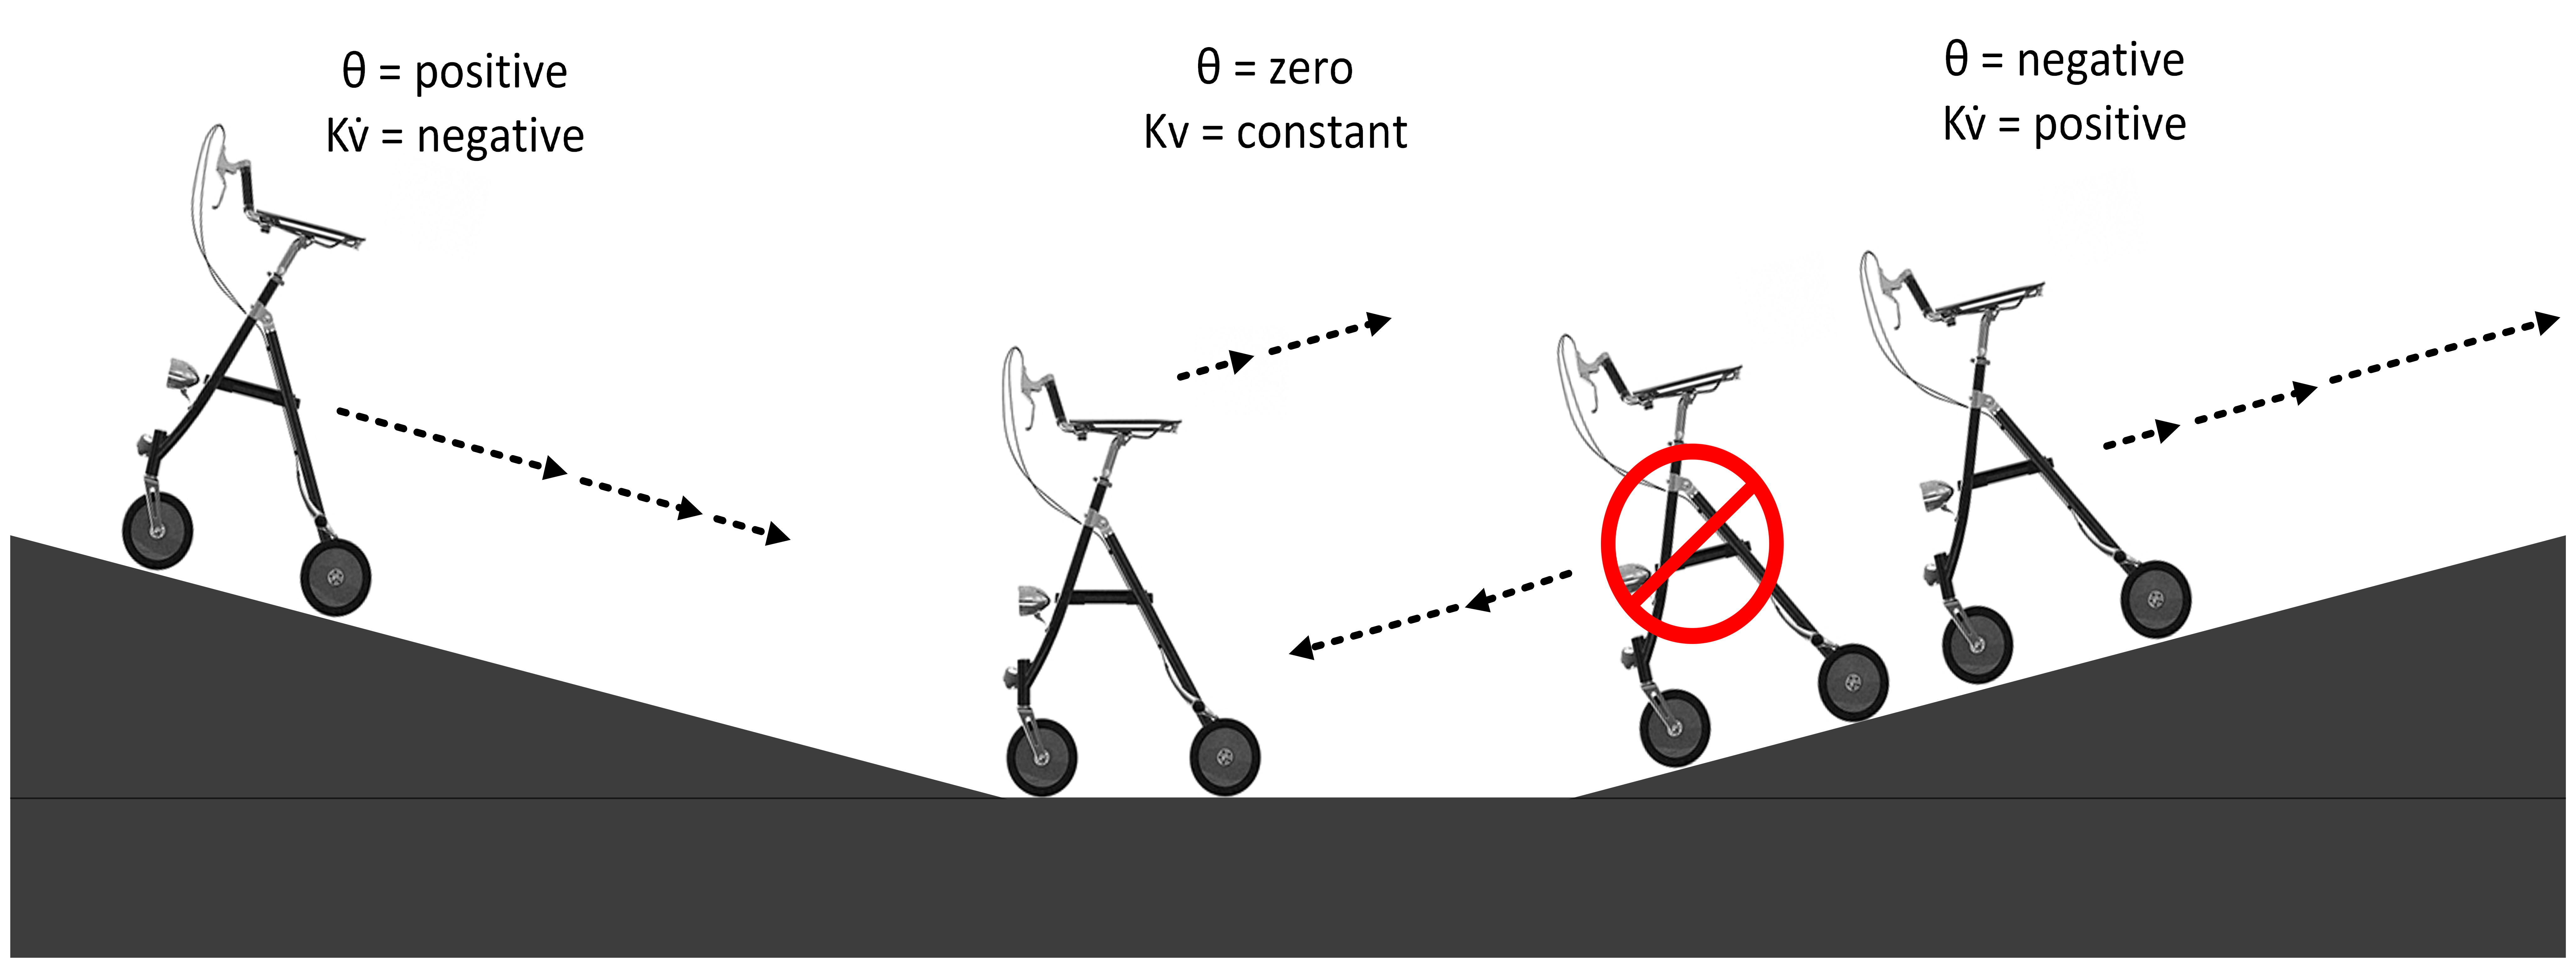
\includegraphics[width=\textwidth]{./Images/Incline-Decline-Stability.png}
	\caption{\label{fig:slope-stability}Stability on Slopes}
\end{figure}
